\subsection{Постановка задачи на разработку программы}
\tab[0.75cm]Программа должна соответствовать требованиям, представленным в 
Техническом 
Задании.

\bigskip
Задачи работы:

\smallskip
\begin{my_enumerate}
\item Реализовать возможность игры в режиме Virtual Reality
\item Реализовать возможность игры в режиме Normal Mode
\item Реализовать возможность передвижения персонажа без задействования 
элементов управления Cardboard'a
\item Реализовать возможность взятия предметов без без задействования 
элементов управления Cardboard'a
\item Реализовать возможность бросить предмет без без задействования 
элементов управления Cardboard'a
\item Реализовать проигрывание звука ходьбы персонажа, звук взятия предметов, 
открытия/закрытия двери, ветра
\item Реализовать показ текста пользователю для отображения необходимой на 
конкретный момент времени информации
\item Реализовать логику головоломок, цепочка решений которых приведет к ключу
\item Реализовать обучающий фрагмент в начале игры, содержащий руководство 
пользователя по управлению в игре
\end{my_enumerate}


\subsection{Описание правил игры}

\tab[0.75cm]Данная игра спроектирована в жанре \textbf{escape the room} (см. 
Приложение - 
Терминология). В таких играх необходимо выбраться из запертого помещения при 
помощи средств, находящихся в самой комнате. Обычно в них есть 
последовательность головоломок, решение которых постепенно приводит к ключу, с 
помощью которого можно будет отпереть дверь и выбраться. Соответственно, 
конечной целью игры является выход из запертого дома при помощи найденного 
ключа.

\subsection{Описание алгоритма и функционирования программы}

\subsubsection{Описание построения игры}
В игре задумано три сцены:
\begin{my_enumerate}
    \item \textbf{ModChooser} Сцена для выбора режима. Является самой первой 
    сценой, которая загружается всегда в Normal Mode. В ней всего 2 кнопки для 
    выбора режима: <<VR Mode>> и <<Normal Mode>>. После нажатия на одну из них, 
    все последующие сцены будут загружаться в выбранном режиме.
    \item \textbf{TransitScene} Сцена, в которой происходит обучение игрока 
    игровой механике и повествуется вкратце сюжет и цель игры. В этой сцене 
    игрок перемещается в дом, в котором будет происходить основная часть игры.
    \item \textbf{HouseInside1} Главная сцена со всеми головоломками. Здесь 
    происходят основные действия: игрок обнаруживает себя запертым внутри дома 
    и решает найти ключ чтобы выбраться. Для этого ему предстоит решить цепочку 
    головоломок, после решения которых он получит ключ и сможет выбраться из 
    заперти.
\end{my_enumerate}


\subsubsection{Переключение между VR Mode и Normal Mode}

\begin{figure}[h!]
    \centering
    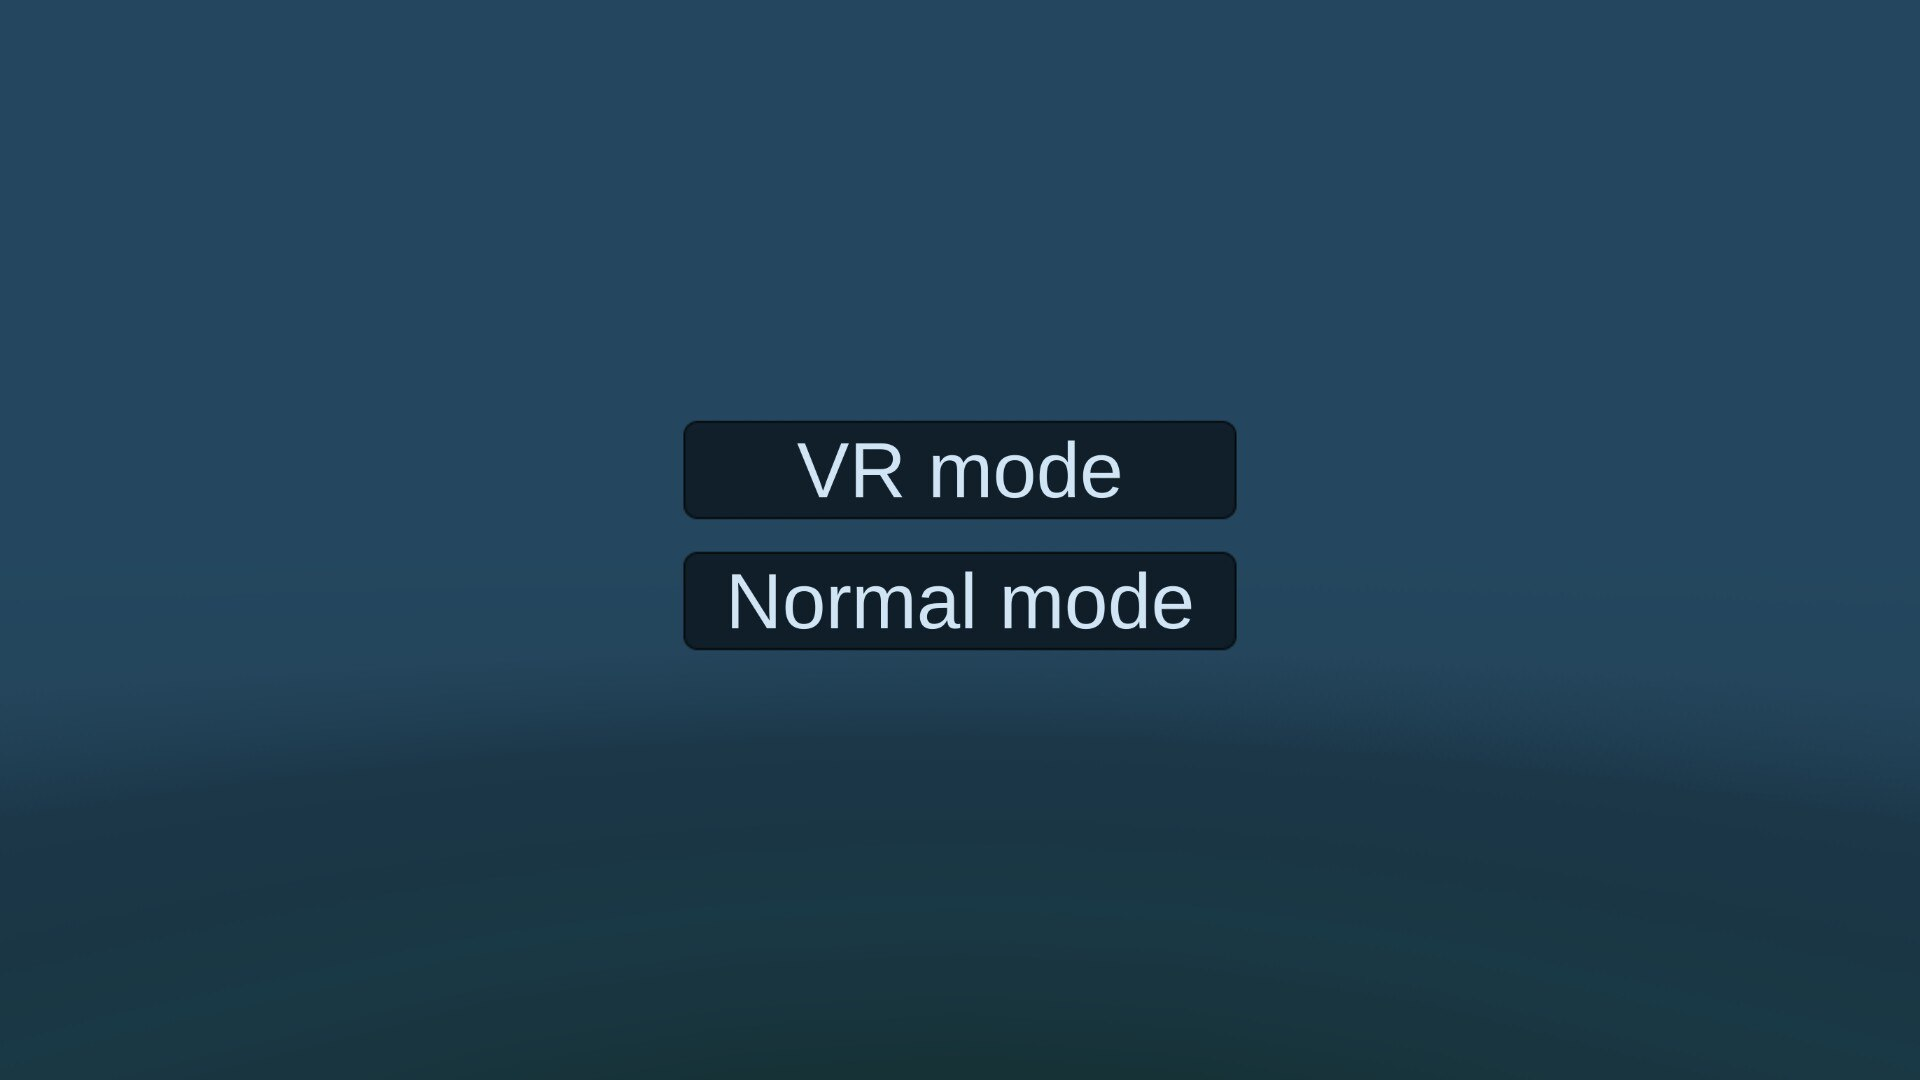
\includegraphics[width=0.8\textwidth]{./screenshots/modes.jpg}
    \caption{\small{меню переключения режима}}
    \label{modes}
\end{figure}

\tab[0.75cm]В любой VR сцене есть объект GvrViewerMain. Этот prefab содержит 
скрипт GvrViewer, который контролирует параметры VR mode. При помощи изменения 
параметра VRModeEnabled на true или false, VR mode будет включен/ выключен 
соответственно. По скольку каждая сцена загружается по умолчанию в VR mode, 
надо запоминать выбор пользователя в начале и при каждой загрузке последующих 
сцен выставлять выбранный режим. Для этого был написан скрипт ModChanger.cs, 
который запоминает выбор игрока.

\begin{figure}[h!]
	\centering
	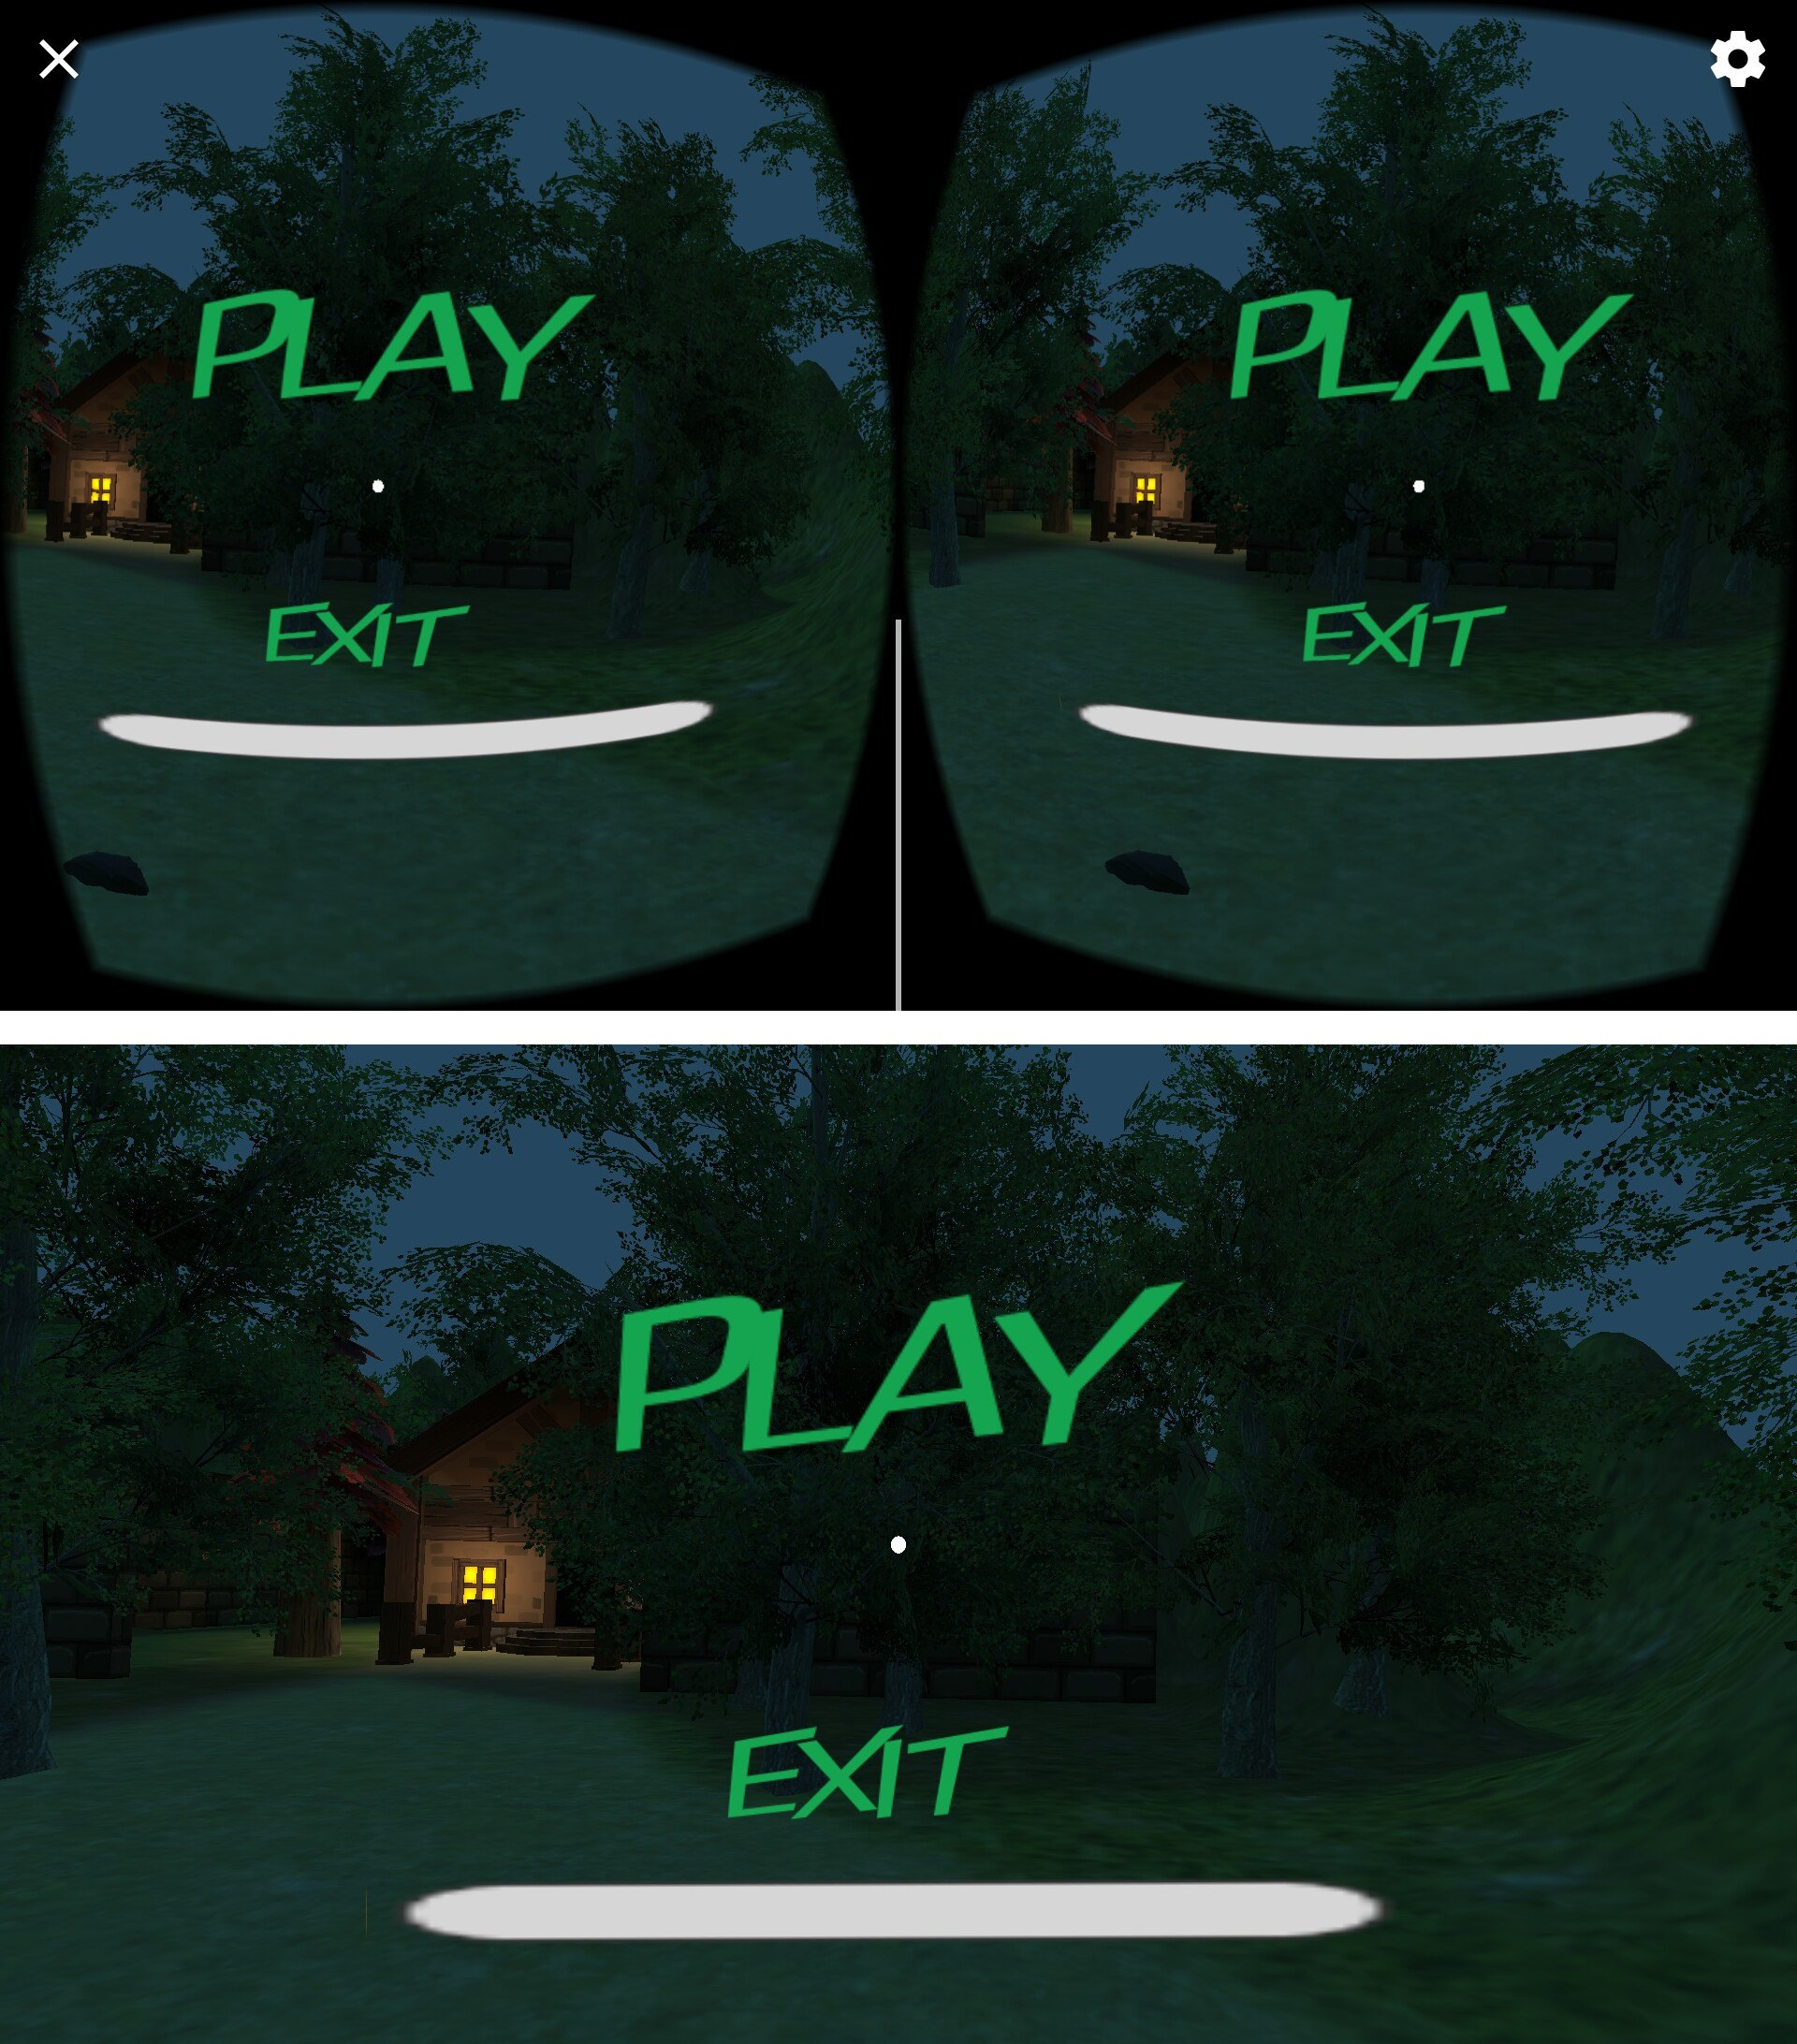
\includegraphics[width=0.8\textwidth]{./screenshots/diff.jpg}
	\caption{\small{разница между VR Mode (сверху) и Normal Mode (снизу)}}
	\label{diff}
\end{figure}
\newpage
\subsubsection{Передвижение игрока без триггера}
\tab[0.75cm]В VR играх передвижение игрока может происходить различными методами. Например, 
есть способ, в котором при нажатии триггера, начинается движение в сторону 
взгляда персонажа, при следующем нажатии на триггер, движение останавливается. 
Поскольку одной из главных задач проекта была разработать игру, в которой не 
задействуется триггер (для совместимости со всеми видами Cardboard), то была 
разработана система передвижения "взглядом".

\newpage

\begin{figure}[h!]
    \centering
    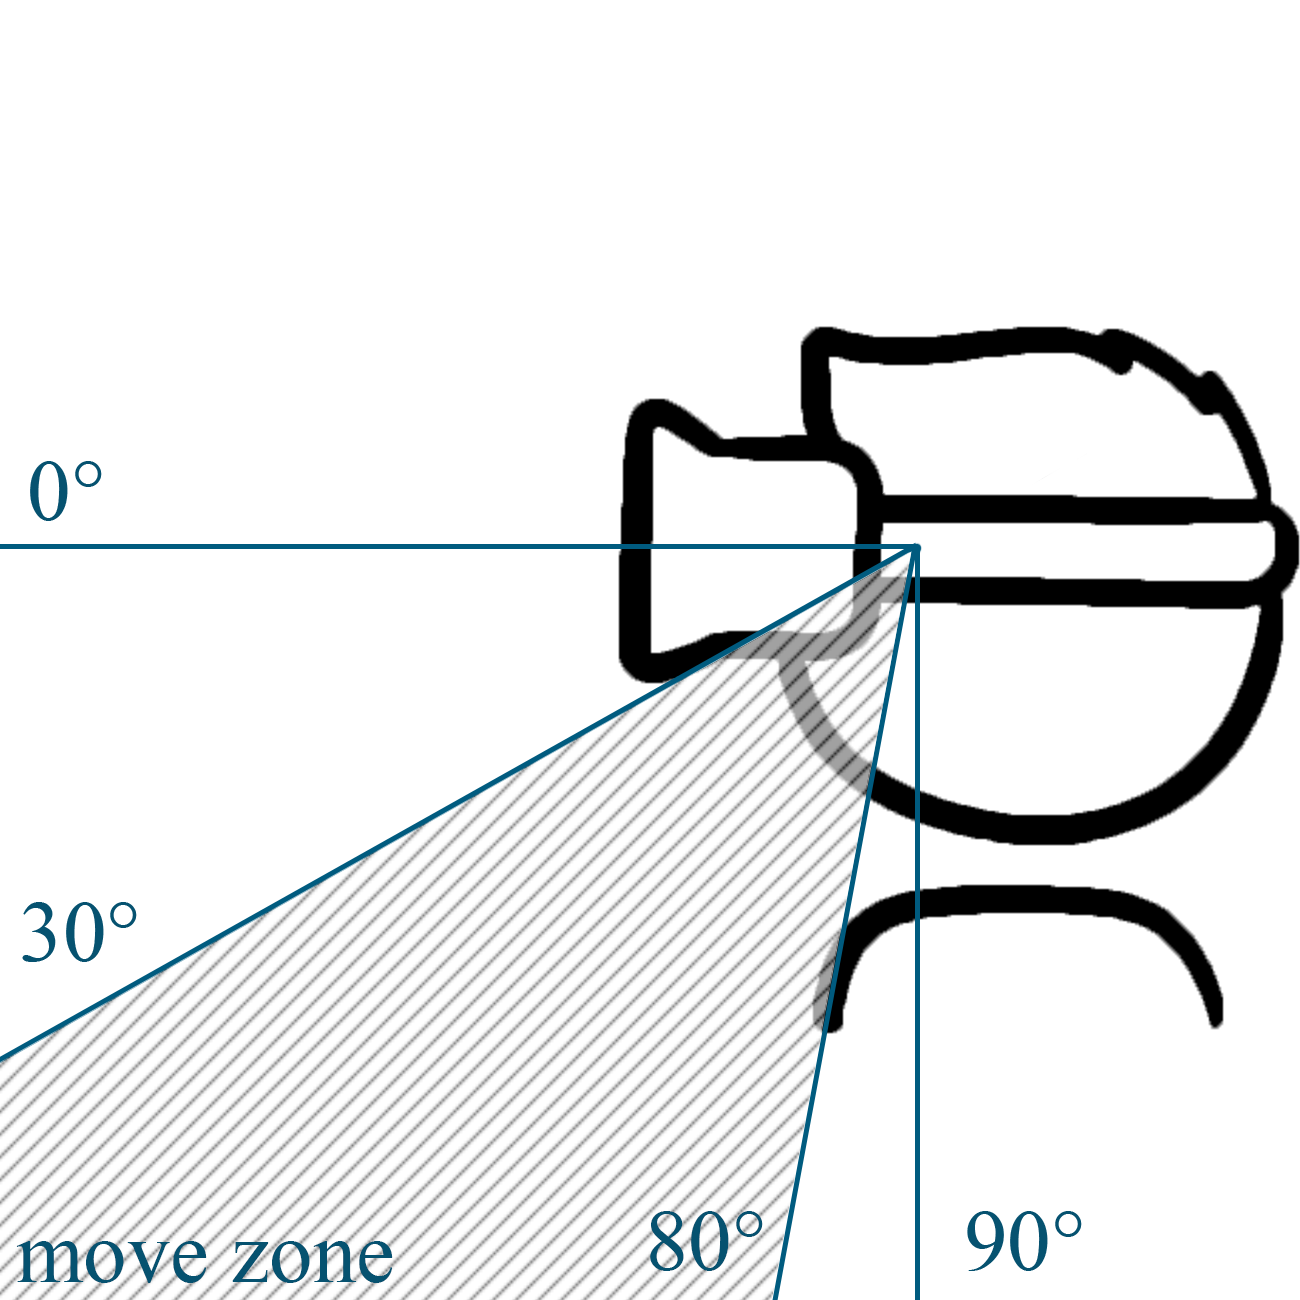
\includegraphics[width=0.7\textwidth]{./pics/vrAngles.png}
    \caption{\small{передвижение при помощи угла взгляда}}
    \label{move_angles}
\end{figure}

\begin{figure}[h!]
    \centering
    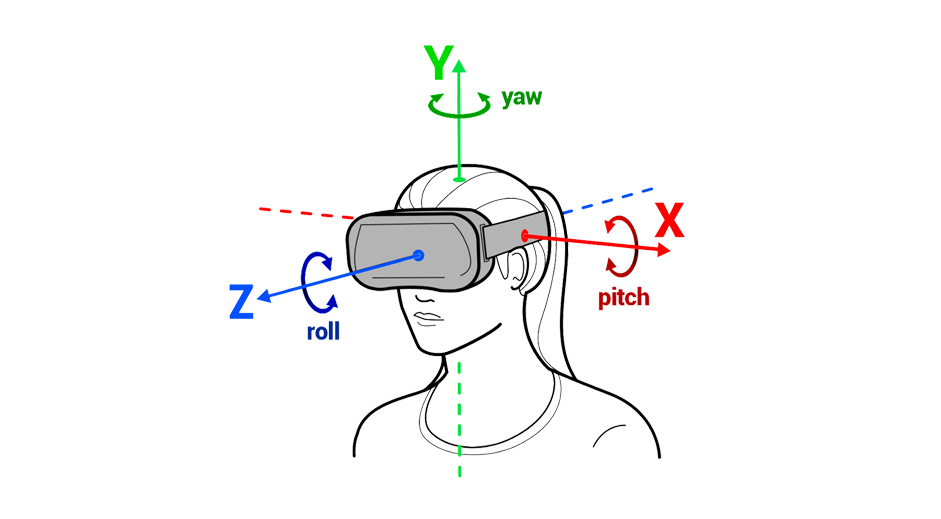
\includegraphics[width=0.8\textwidth]{./pics/angles.png}
    \caption{\small{расположение осей в виртуальной реальности}}
    \label{axes}
\end{figure}

На схеме(рис. \ref{move_angles}) видно, что при достижении угла от 30\degr до 80\degr по оси Х (см. 
рис. \ref{axes})
происходит движение игрока. Движение происходит в сторону направления взгляда 
(вперед).

Ниже приведен Update метод скрипта WalkByLook.cs. Любой Update метод в юнити вызывается раз за фрейм.

\begin{small}
	\begin{verbatim}
void Update()
{
    shouldMove = false;
    mustLookToTheObject = GazeInputModule.pointingAt != null;
    if (mustLookToTheObject && GazeInputModule.pointingAt.Count > 0)
        lookingToObject = (((bool)GazeInputModule.pointingAt[1] && 	(float)GazeInputModule.pointingAt[2] >= 4F)
        || !((bool)GazeInputModule.pointingAt[1]));

    moveForward = (vrCam.eulerAngles.x >= angle1 && vrCam.eulerAngles.x <= angle2);

    if (moveForward && (!mustLookToTheObject || (mustLookToTheObject && lookingToObject)))
    {
        shouldMove = true;
        Vector3 forward = vrCam.TransformDirection(Vector3.forward);
        cc.SimpleMove(forward * speed);
        if (!playing)
            StartCoroutine(PlaySteps());
    }
}
	\end{verbatim}
\end{small}


\subsubsection{Взаимодействие предметов без триггера}

\tab[0.75cm]В VR играх взаимодействие с предметами происходит различными методами. Например, при нажатии на триггер, предмет перемещается в руку персонажа или перемещается в инвентарь. Поскольку одной из главных задач проекта была разработать игру, в которой не 
задействуется триггер (для совместимости со всеми видами Cardboard), то была 
разработана система взаимодействия с объектами "взглядом".

При наведении reticle (прицела) на объект, над которым может быть совершено действие, полоса загрузки внизу экрана активируется и по ее заполнению произойдет действие над объектом. Это может быть, например, взятие его в руку (см рис. \ref{pick_stone}, рис. \ref{picked_stone}).

\begin{figure}[h!]
	\centering
	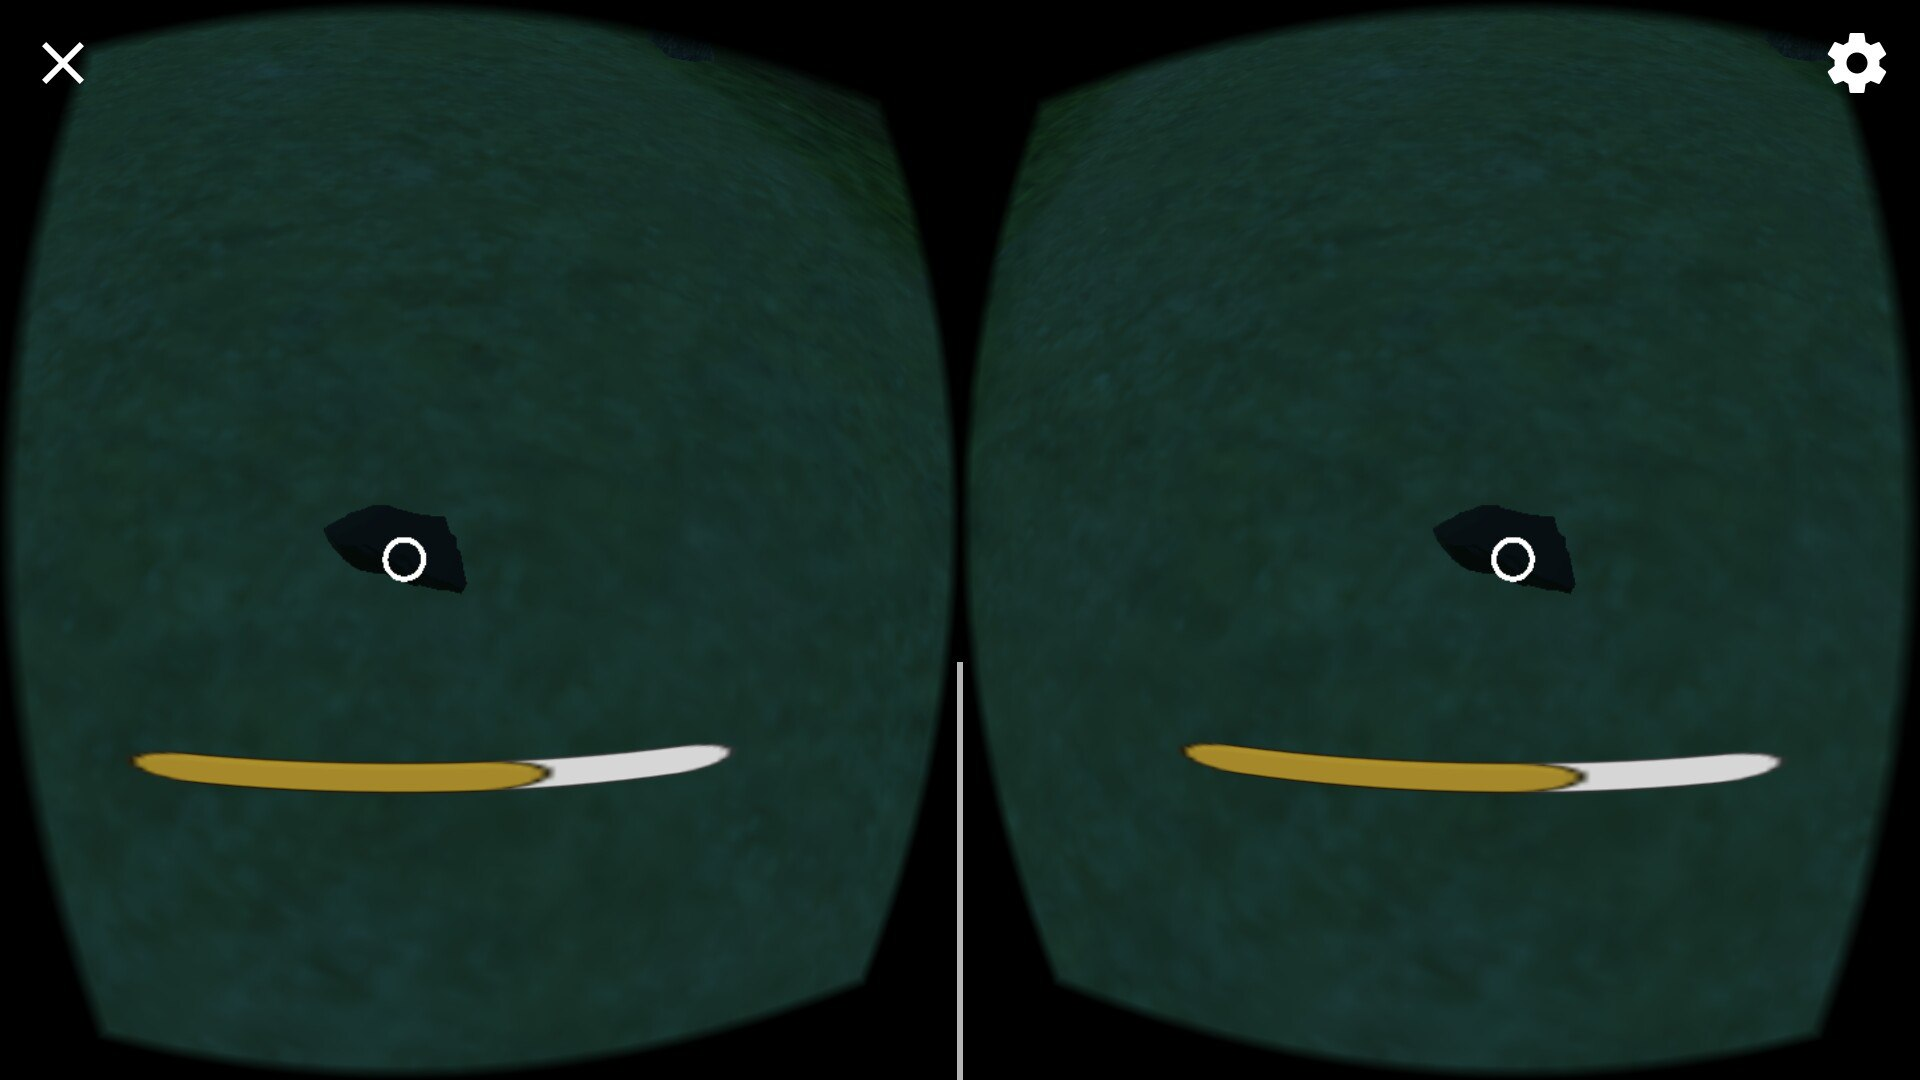
\includegraphics[width=0.6\textwidth]{./screenshots/pick_stone1.jpg}
	\caption{\small{ожидание выполнения действия над объектом камень}}
	\label{pick_stone}
\end{figure} 

\begin{figure}[h!]
	\centering
	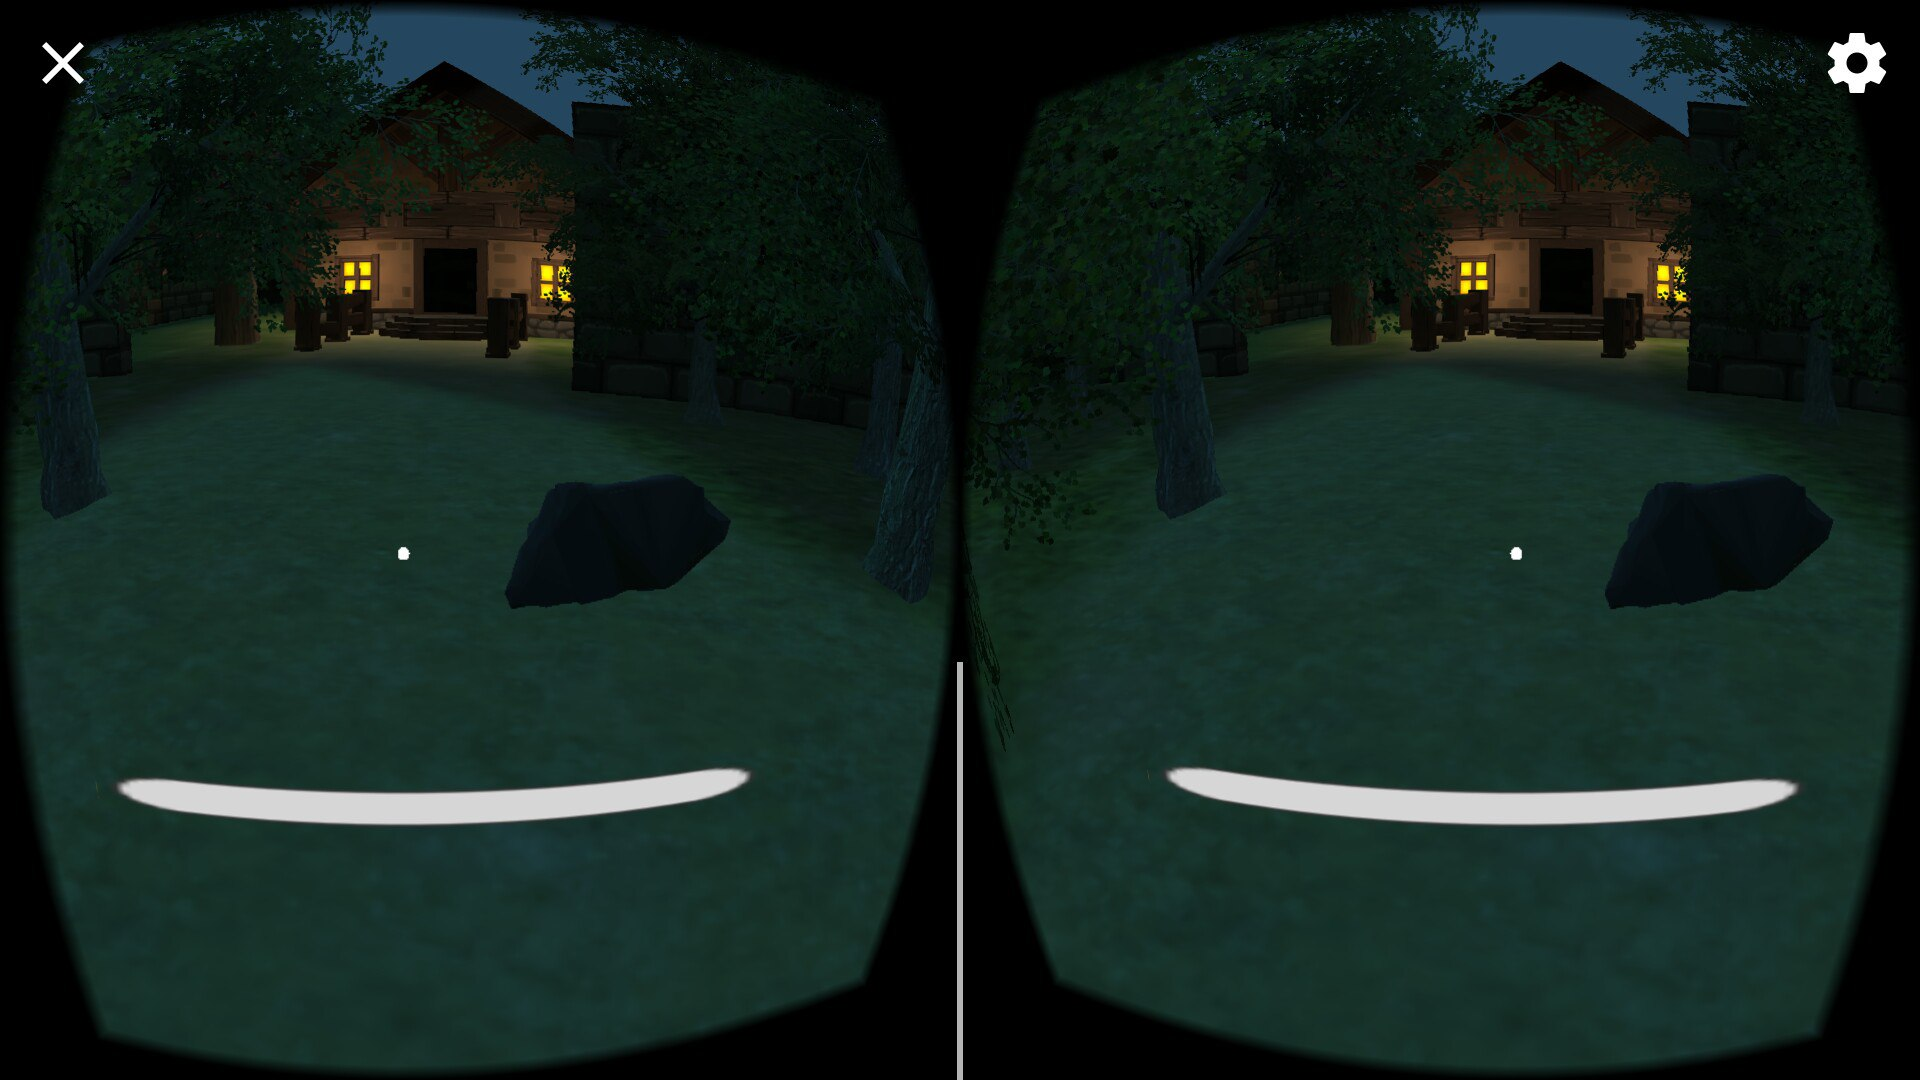
\includegraphics[width=0.8\textwidth]{./screenshots/picked_stone1.jpg}
	\caption{\small{результат выполнения действия над объектом - камень в руке}}
	\label{picked_stone}
\end{figure} 

\tab[0.75cm]Поскольку при взгляде на объект часто бывает, что угол наклона камеры попадает в приемлемую для передвижения зону(от 30\degr до 80\degr), то в скрипте WalkByLook.cs предусмотрена остановка передвижения при взгляде на объект, над которым можно совершить действие. Это позволяет брать предметы "на ходу". 

\subsubsection{Перемещение предметов в руку}

\tab[0.75cm]Поднятый предмет перемещается в руку путем изменения его положения на равное положению руке. Рука - невидимый игровой объект, расположенный относительно персонажа (подсвечен фиолетовым) как на рис. \ref{hand}. Относительно игрока рука расположена как на рисунке \ref{picked_stone}.

\begin{figure}[h!]
	\centering
	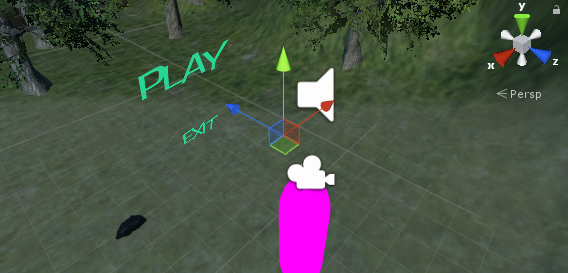
\includegraphics[width=0.8\textwidth]{./screenshots/hand.png}
	\caption{\small{расположение руки относительно персонажа (подсвечен фиолетовым)}}
	\label{hand}
\end{figure} 

За процесс поднятия предмета отвечает скрипт PickUpObject. При вызове метода MoveToPlayersHand() предмет, к которому прикреплен скрипт переместится в руку персонажа. Так же здесь сохраняются исходные пропорции объекта, поскольку при изменении родителя (а тут объект переходит от одного родителя к handMountingPosition) меняются пропорции объекта (особенность Unnity). Пока предмет находится в руке у него отключаются RigidBody и Collider для предотвращения столкновения с окружающей средой. В последствии при броске предмета они включаются обратно. В дополнение к этому у каждого предмета в этом скрипте задана позиция и вращение руки, которое необходимо ей придать при поднятии объекта (handPosition и handRotation). Это нужно для того, чтобы предмет, например, ключ, не был направлен обратной стороной к двери при попытки открыть ее им. Ниже приведен метод MoveToPlayersHand(). Этот скрипт также отвечает за проигрывание звука взятия предмета.

\begin{small}
	\begin{verbatim}
    public void MoveToPlayersHand()
    {
        if (!pickedUp)
        {
            vrCam.parent.GetComponents<AudioSource>()[0].Play();
            oldScale = gameObject.transform.localScale;
            gameObject.transform.parent = handMountingPosition;
            gameObject.GetComponent<Rigidbody>().useGravity = false;
            gameObject.GetComponent<Rigidbody>().isKinematic = true;
            gameObject.GetComponent<Collider>().enabled = false;
            gameObject.GetComponent<Rigidbody>().constraints = new RigidbodyConstraints();
            gameObject.transform.localScale = oldScale;
            
            gameObject.transform.localPosition = new Vector3(0F, 0F, 0F);
            gameObject.transform.localRotation = Quaternion.Euler(0F, 0F, 0F);
            handMountingPosition.localRotation = Quaternion.Euler(handRotation);
            handMountingPosition.localPosition = handPosition;
            handMountingPosition.localScale = new Vector3(1F, 1F, 1F);
        }
    }
	\end{verbatim}
\end{small}


Этот же скрипт отвечает за бросание предметов. При положении камеры (головы игрока) от 275\degr до 303\degr вызывается метод ThrowObject(), его код приведен ниже. В нем проигрывается аудио бросания предмета, включаются RigidBody и Collider у объекта и родителем становится null.

\begin{small}
    \begin{verbatim}
    public void ThrowObject()
    {
        if (pickedUp && handMountingPosition.GetChild(0).name.CompareTo(gameObject.name) == 0)
        {
            vrCam.parent.GetComponents<AudioSource>()[0].Play();
            gameObject.GetComponent<Rigidbody>().useGravity = true;
            gameObject.GetComponent<Rigidbody>().isKinematic = false;
            gameObject.GetComponent<Collider>().enabled = true;
            gameObject.transform.parent = null;
            gameObject.transform.localScale = oldScale;
        }
    }
    \end{verbatim}
\end{small}

\subsubsection{Модификация исходников Google VR SDK}

\tab[0.75cm]В процессе написания программы были выявлены проблемы при использовании скрипта GazeInputModule, предоставляемым в SDK от Google для VR приложений. Проблема заключалась в том, когда камера светит лучем вперед для того чтобы получить первый объект, который он ударит, он упирался в самого персонажа и видел дальше него лишь иногда (непредсказуемое поведение). См. рис. \ref{problem}.

\begin{figure}[h!]
    \centering
    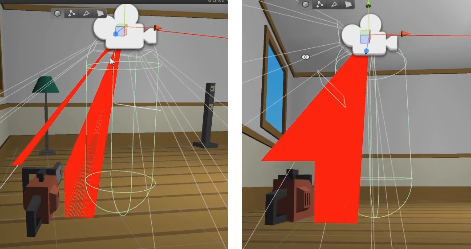
\includegraphics[width=0.5\textwidth]{./screenshots/problem1.png}
    \caption{\small{Debug режим. Проблема при использовании оригинального скрипта от Google GazeInputModule.cs. Слева - до, справа - после внесения модификаций в скрипт.)}}
    \label{problem}
\end{figure} 


Изменения приняли следующий вид. В методе CastRayFromGaze(), который <<стреляет лучем>>, чтобы получить объект, на который в данный момент указывает камера, был добавлен следующий код:

\begin{small}
    \begin{verbatim}
    ...
    if (pointerData.pointerCurrentRaycast.gameObject != null)
        if (pointerData.pointerCurrentRaycast.gameObject.name.CompareTo("Character") == 0)
            if (m_RaycastResultCache.Count > 1)
                pointerData.pointerCurrentRaycast = m_RaycastResultCache[1];
            else
        pointerData.Reset();
    ...
    \end{verbatim}
\end{small}

После того, как был взят первый объект, с которым столкнулся луч, он проверяется на равенство null. Затем, если это сам персонаж, то берется следующий объект за персонажем, который ударила камера. На рисунке \ref{problem} видно, что после внесения изменений, камера стала видеть весь Collider формы прямоугольного параллелепипеда корректно. 

Далее, при условии, что текущий GameObject не null, формируется статичесикй массив pointingAt из трех объектов для получения дополнительных данных из просвечивания объектов лучем:
\begin{itemize}
    \item [0] - сам GameObject
    \item [1] - hasEventTrigger. Интерактивный ли это объект. В зависимости от этого параметра определяется будет ли происходить взаимодействие с объектом или нет
    \item [2] - distance. Расстояние до объекта
\end{itemize}

\begin{small}
    \begin{verbatim}
    float distance = Vector3.Distance(pointerData.pointerCurrentRaycast.gameObject.transform.position, vrCam.transform.position);
    bool hasEventTrigger = pointerData.pointerCurrentRaycast.gameObject.GetComponent<EventTrigger>()s
     as EventTrigger != null;
    
    pointingAt.Add(pointerData.pointerCurrentRaycast.gameObject);
    pointingAt.Add(hasEventTrigger);
    pointingAt.Add(distance);
    \end{verbatim}
\end{small}

Далее, было решено сделать объекты интерактивными на определенном расстоянии. Поскольку неправильно и не логично было бы взаимодействовать с объектом, который находится в одном углу комнаты, находясь в другом. Поэтому было выбрано расстояние 4.35. Дальше него камера пусть и пускает лучи, но в результат ничего не записывает. 

\begin{small}
    \begin{verbatim}
    
    ...
    if (!(distance <= 4.35F && hasEventTrigger))
    {
    pointerData.pointerCurrentRaycast = new RaycastResult();
    m_RaycastResultCache.Clear();
    }
    ...
    \end{verbatim}
\end{small}


\subsubsection{Описание головоломок внутри комнаты}
\tab[0.75cm]Конечная цель игры - найти ключ от двери и выбраться из заперти. Ключ игроку открывается после решения головоломки с цифрами на правой книжной полке. Код от нее спрятан за картиной, которая висит справа от второй кровати и появляется после решения головоломки с колокольчиками. Чтобы решить головоломку с колокольчиками, необходимо чтобы на стене между двумя кроватями висели все 5 колокольчиков. Намек на это есть в записке на столе. Один колокольчик можно найти в котле справа от входа, второй висит над входной дверью, его необходимо открутить при помощи отвертки, которая находится на левой книжной полке. 

Откручивание отверткой колокольчика реализовано в скрипте Uscrew.cs, его код:


\begin{small}
    \begin{verbatim}
    bool unscrewed = false, hasScrewDriver = false;
    public Transform handMountingPosition;

    void Update()
    {
        if (handMountingPosition.childCount > 0)
            hasScrewDriver = handMountingPosition.GetChild(0).name.Contains("ScrewDriver");
    }
    
    public void PointerClick()
    {
        if (!unscrewed && hasScrewDriver)
        {
            gameObject.SetActive(false);
            gameObject.GetComponent<BoxCollider>().enabled = false;
            GameObject.Find("InnerBell").GetComponent<Rigidbody>().constraints = new RigidbodyConstraints();
            unscrewed = true;
        }
    }
    \end{verbatim}
\end{small}

В Update() проверяется наличие отвертки в руке персонажа, а в PointerClick() у колокольчика отключаются constraints, что держат его на месте, и он падает (рис. \ref{full_unscrew}).


\begin{figure}[h!]
    \centering
    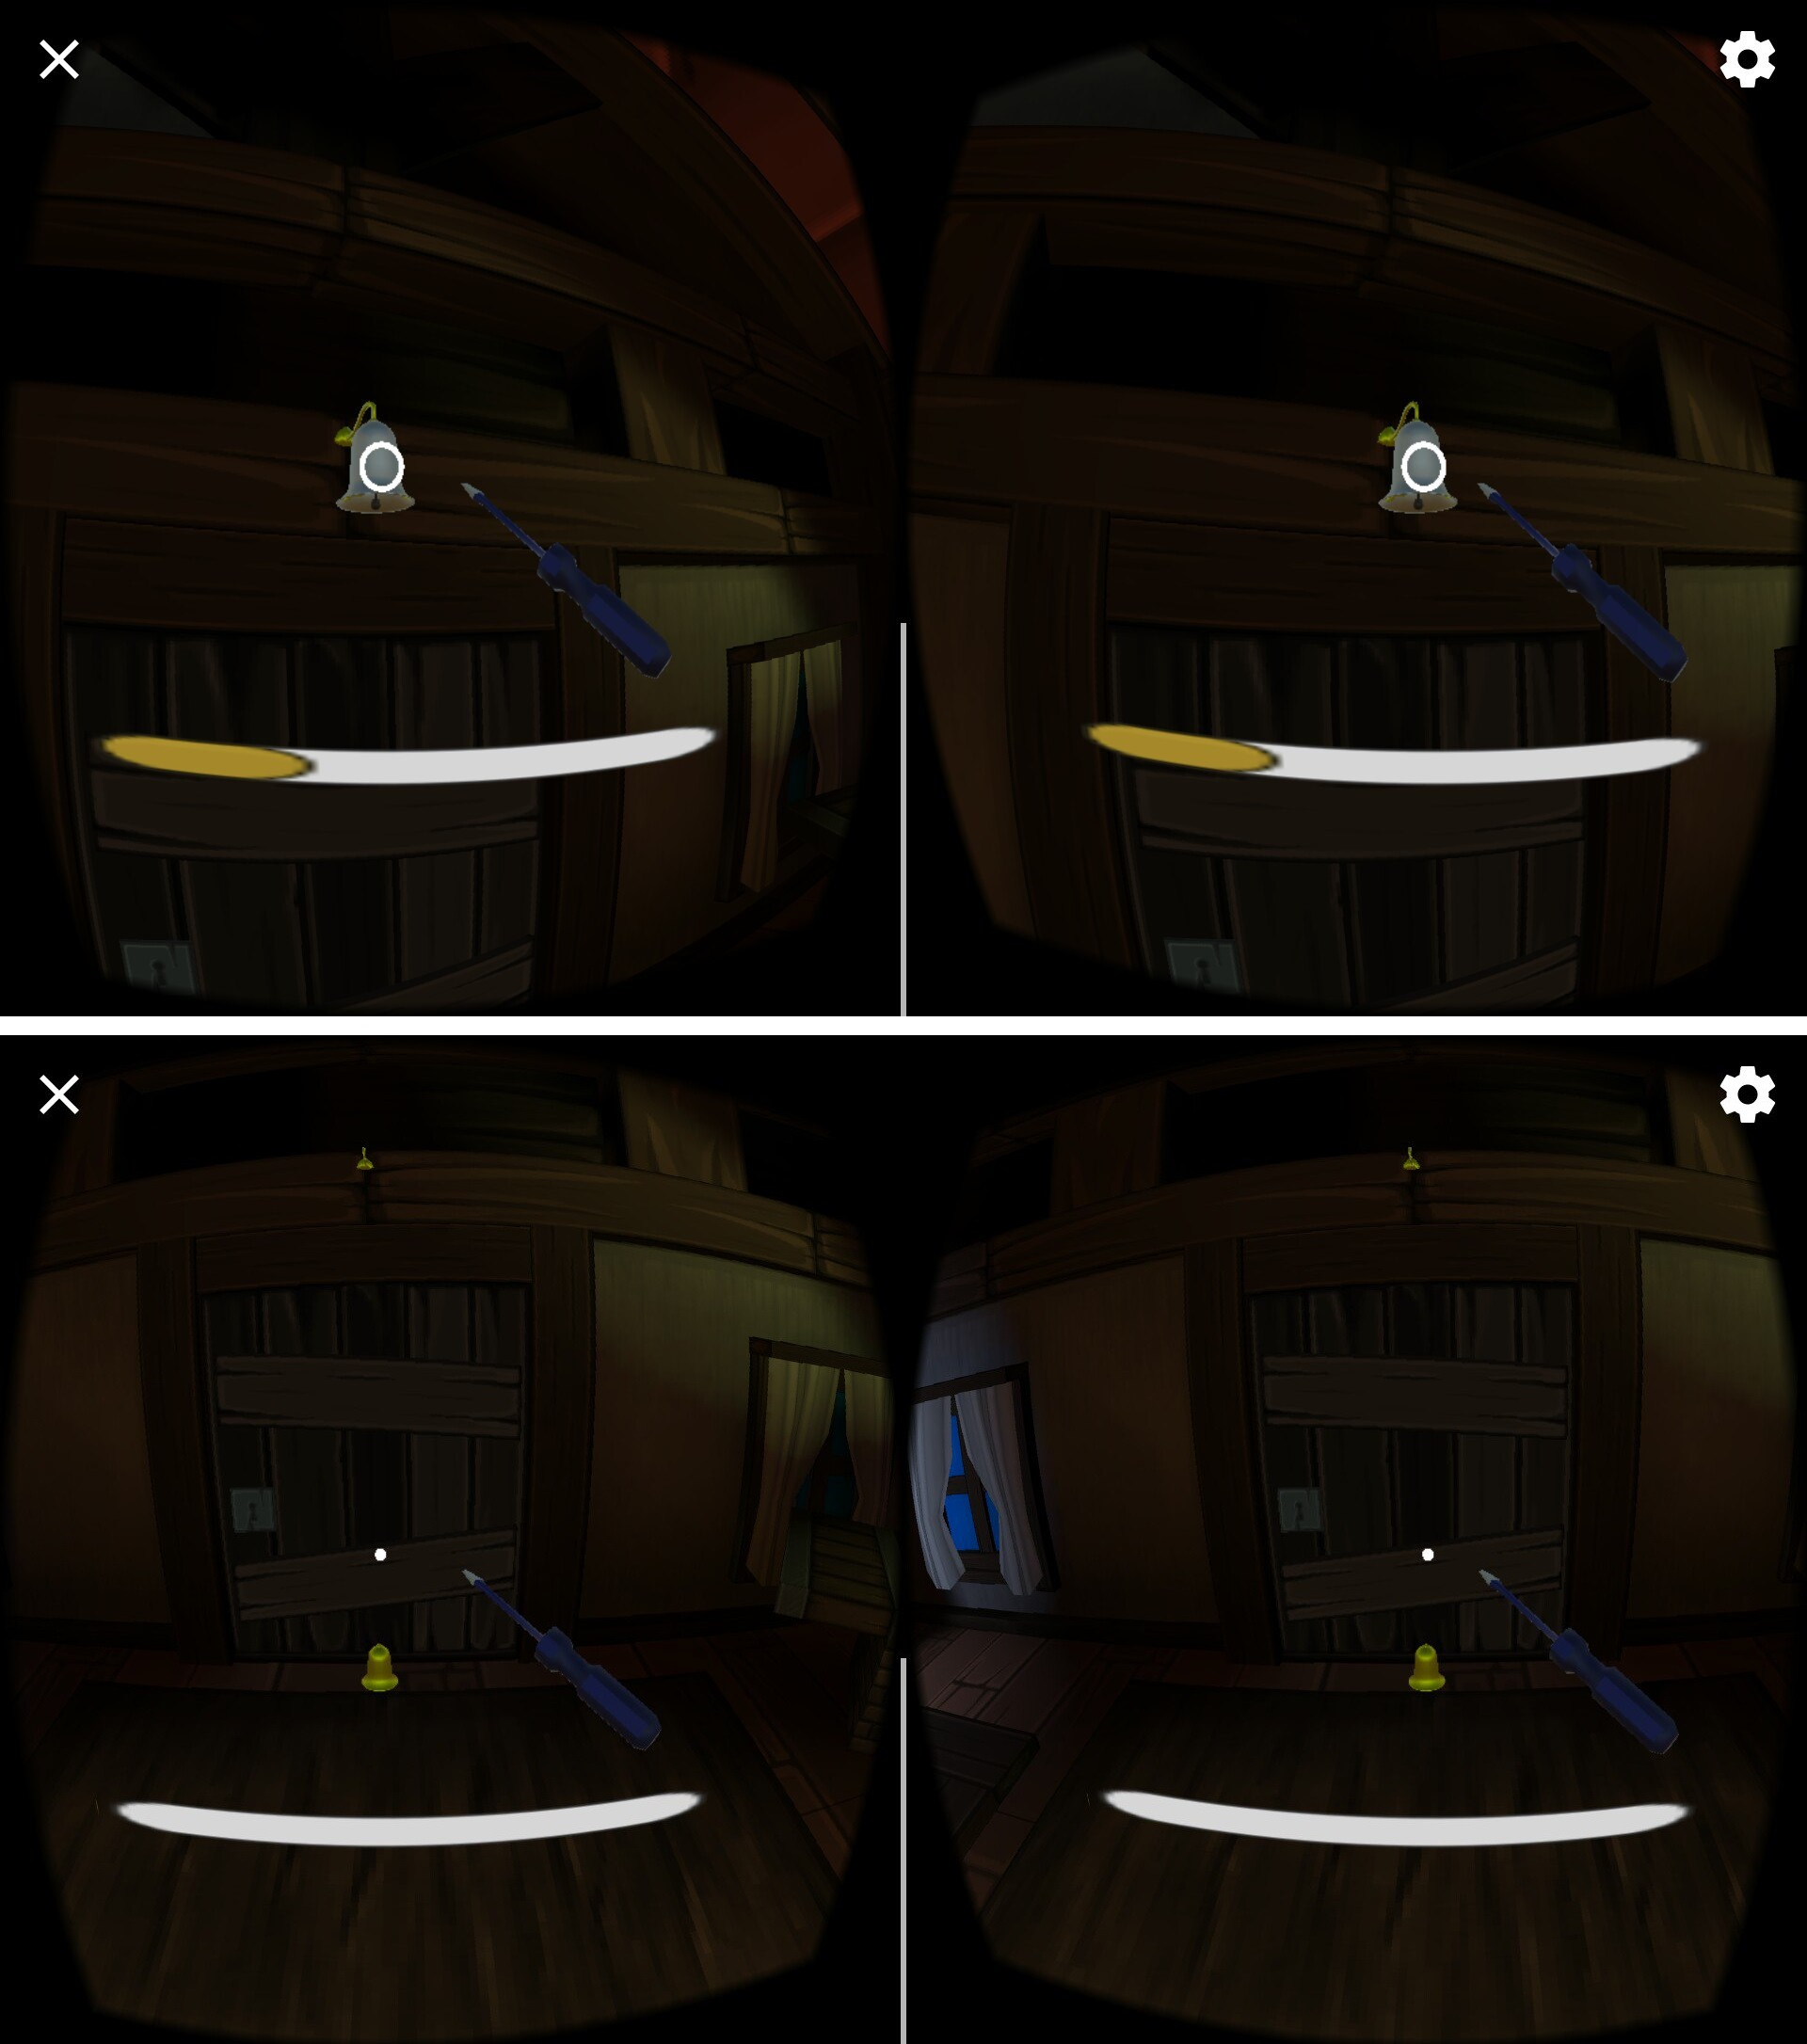
\includegraphics[width=0.8\textwidth]{./screenshots/full_unscrew.jpg}
    \caption{\small{откручивание колокольчика при помощи отвертки. Сверху - сам процесс, снизу - результат.}}
    \label{full_unscrew}
\end{figure} 

Когда все 5 колокольчиков висят на месте, сразу же начнется следующая головоломка. Основная и самая сложная. Заключается она в том, что сначала проигрывается последовательность (5 раз бьют по разным колокольчикам), а затем, игрок должен ее повторить, ударив по тем же колокольчикам, что были показаны.

За данную головоломку отвечает скрипт BellPuzzleLogic.cs. Сначала показывается паттерн сгенерированной последовательности, затем игрок может начинать вводить свою. При очередном неверном выборе колокольчика, подается звуковой сигнал, значащий, что был сделан неверный выбор и произойдет показ паттерна снова.

При верном вводе всей последовательности подается особый звуковой сигнал, означающий, что задание пройдено. Производится визуальный переход ко второму. Появляется и подсвечивается фиолетовыми частицами картина справа (рис. \ref{pic}).

\begin{figure}[h!]
    \centering
    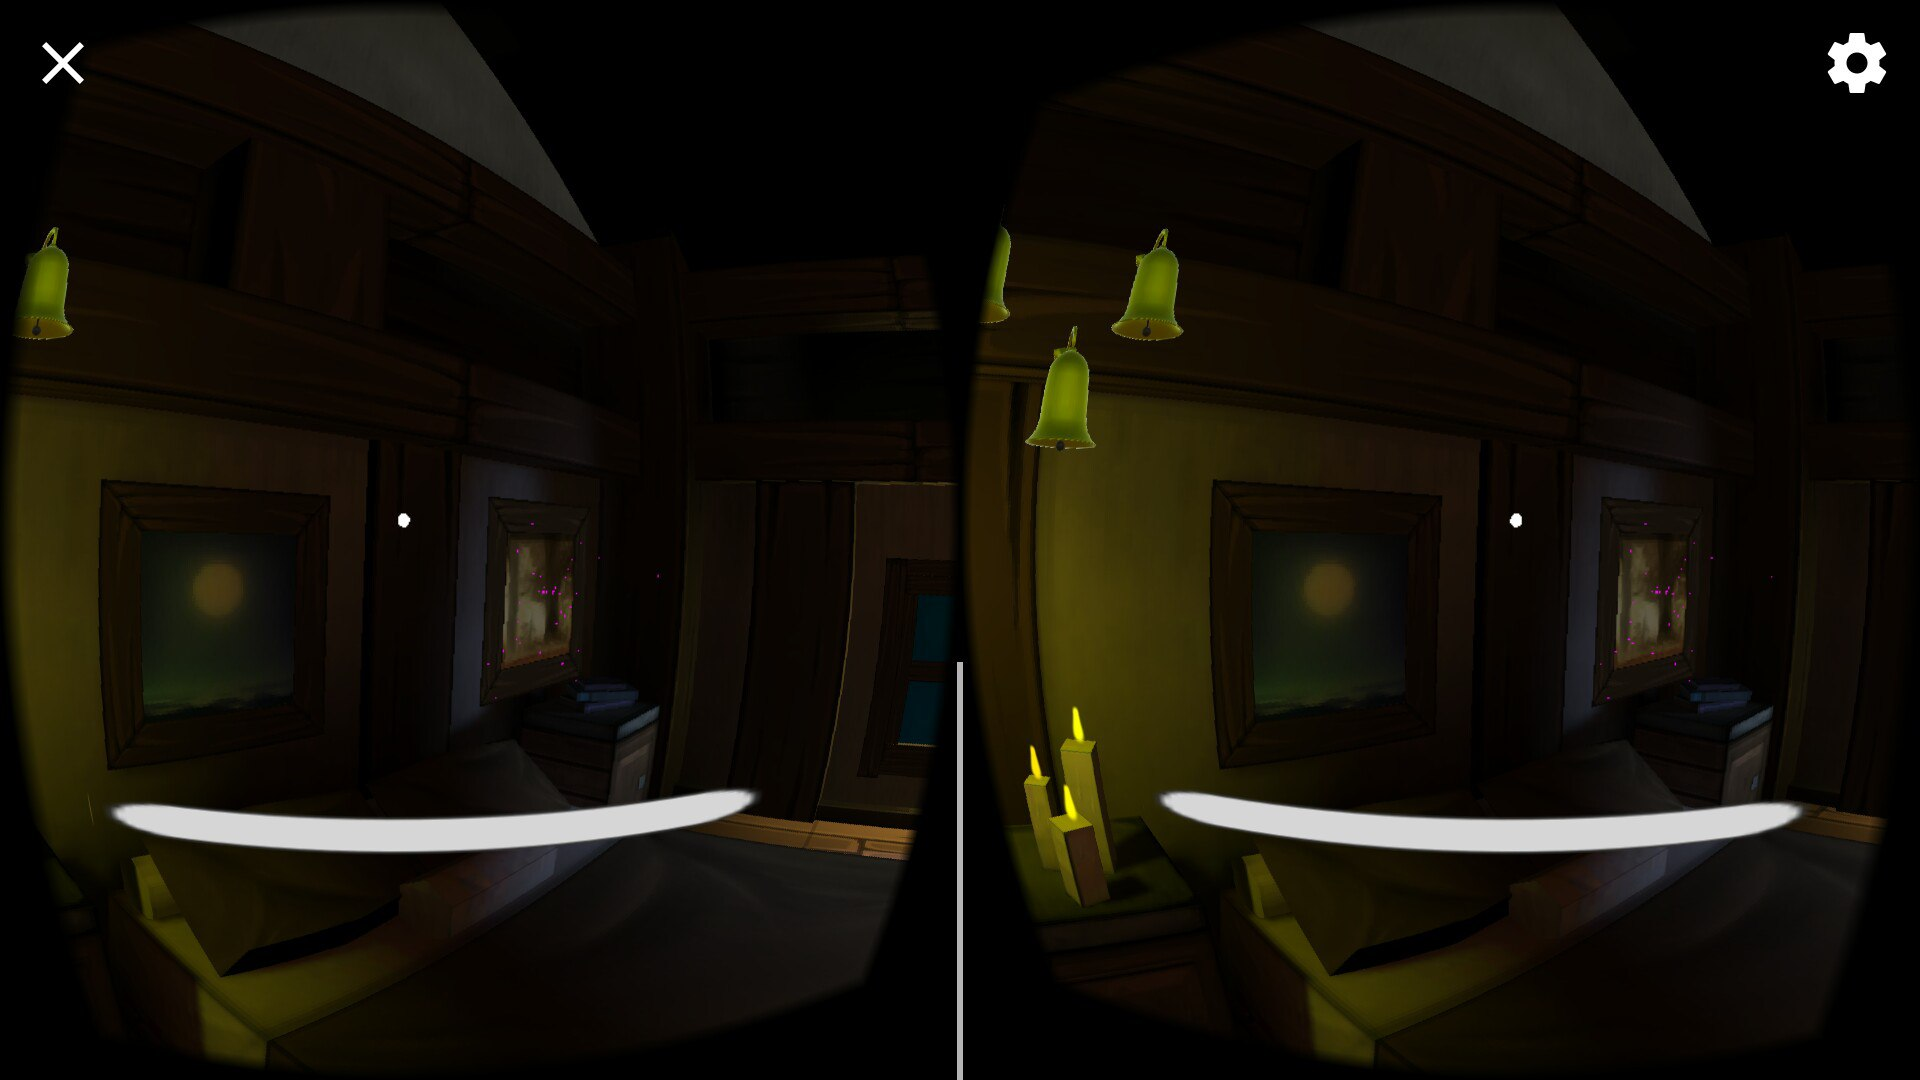
\includegraphics[width=0.8\textwidth]{./screenshots/pic.jpg}
    \caption{\small{появившаяся картина после завершения задания с колокольчиками.}}
    \label{pic}
\end{figure} 


За картиной находится код. Игрок  должен запомнить его. Рис (\ref{code}).

\begin{figure}[h!]
    \centering
    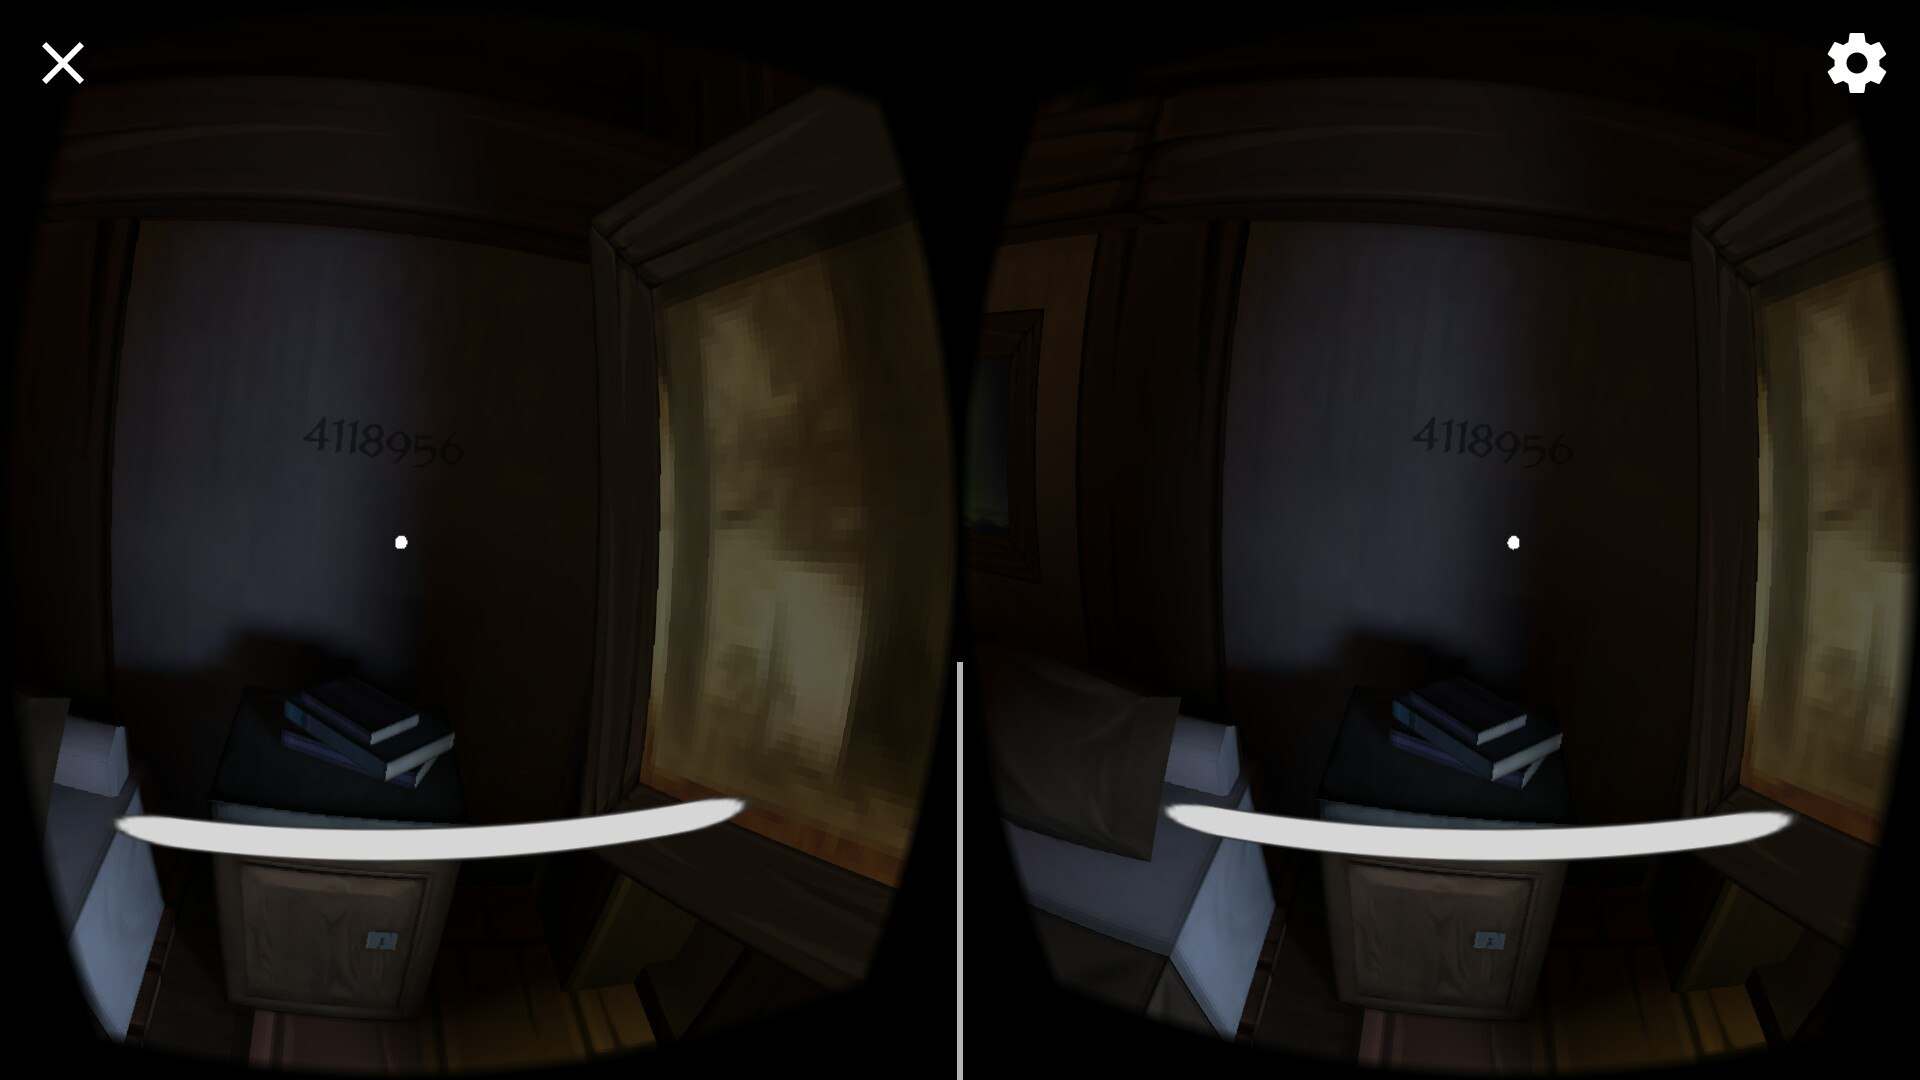
\includegraphics[width=0.8\textwidth]{./screenshots/code.jpg}
    \caption{\small{код дл финальной головоломки за картиной.}}
    \label{code}
\end{figure} 

\begin{figure}[h!]
    \centering
    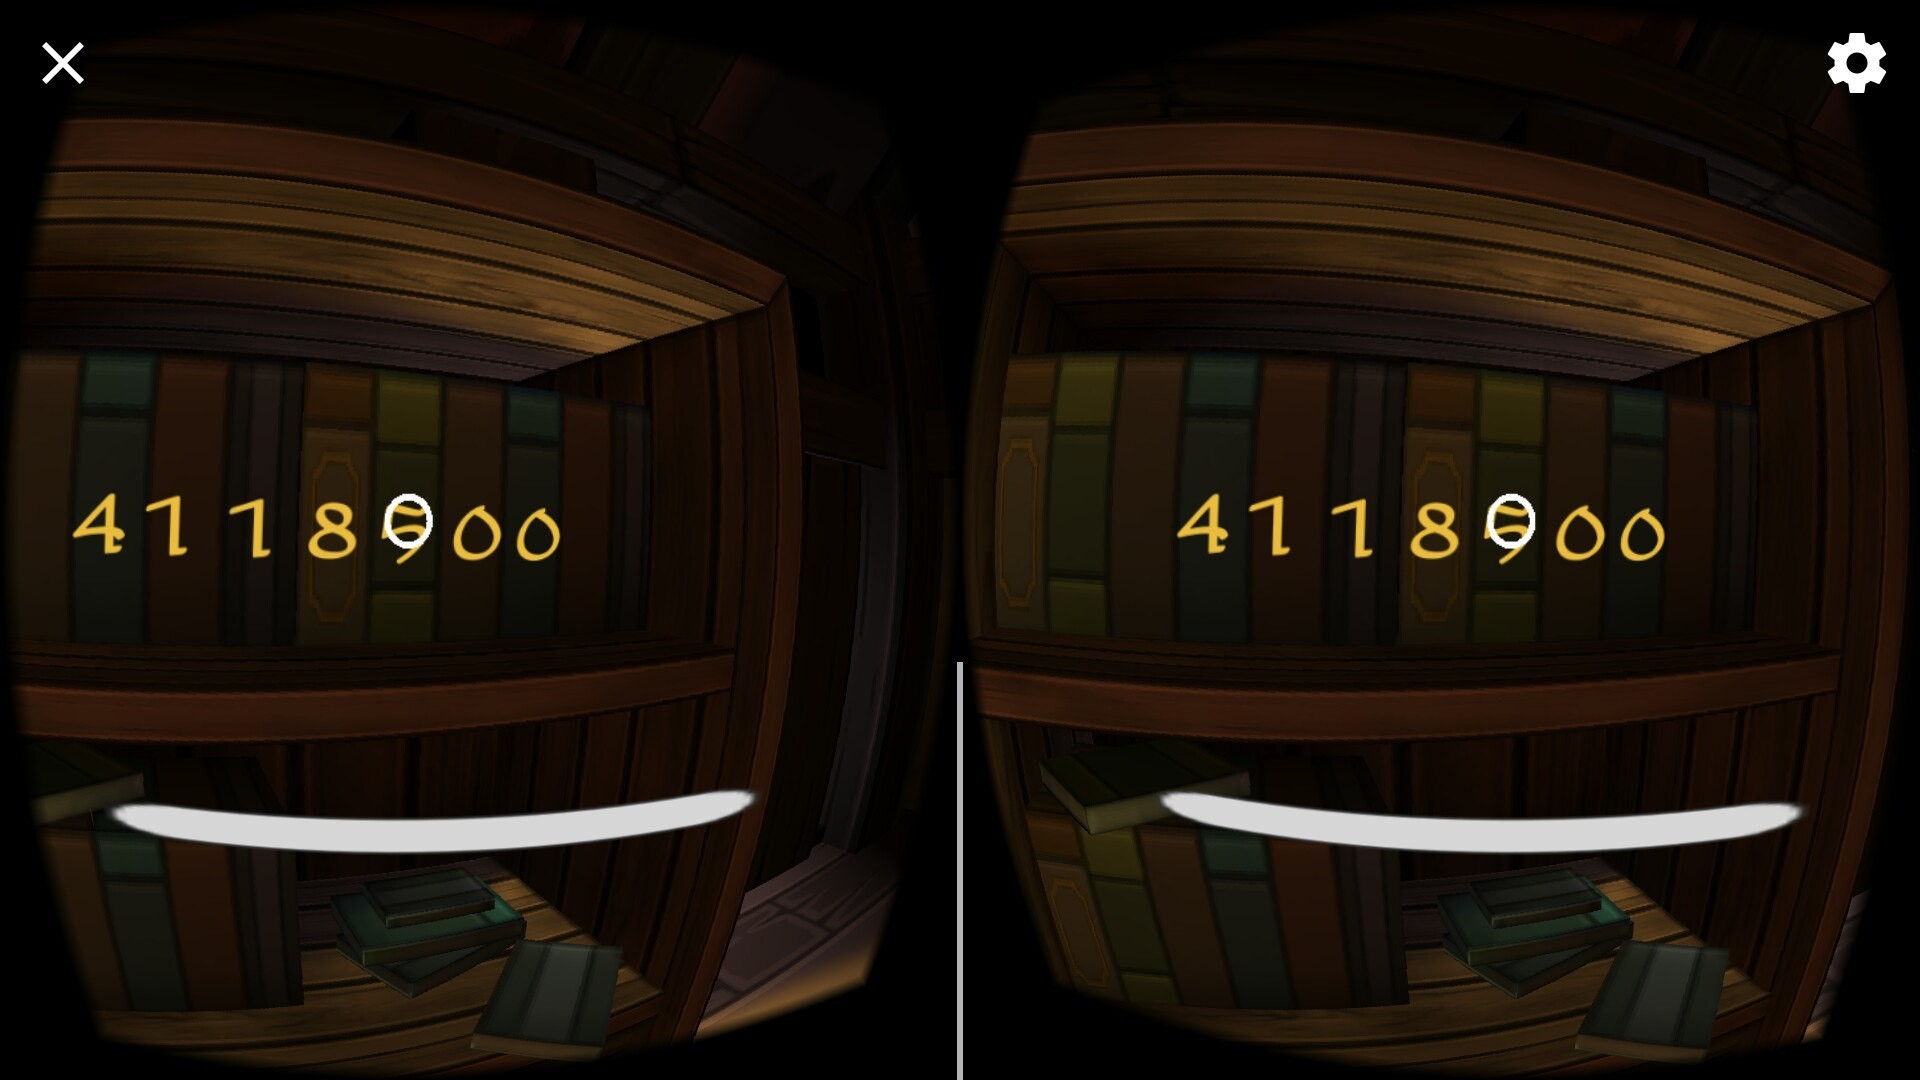
\includegraphics[width=0.8\textwidth]{./screenshots/last_code.jpg}
    \caption{\small{ввод кода для получения ключа.}}
    \label{last_code}
\end{figure} 

\newpage
Финальная задача состоит в том, чтобы ввести полученный код в поле, находящееся на правом книжном шкафу. 
В скрипте LastPuzzleLogic.cs расположен код для последней задачи. Здесь при вводе очередной цифры пользователем последовательность проверяется на соответствие правильному ключу:

\begin{small}
    \begin{verbatim}
void Start()
{
    solved = false;
    numbers = new char[7];
}

void Update()
{
    if (!solved)
    {
        int i = 0;
        foreach (Transform child in transform)
        {
            numbers[i] = child.GetComponent<TextMesh>().text[0];
            ++i;
        }
        
        if (new String(numbers).CompareTo(key) == 0)
        {
            solved = true;
            Key.SetActive(true);
            Key.GetComponent<Rigidbody>().constraints = new RigidbodyConstraints();
            gameObject.SetActive(false);
        }
    }
}
    \end{verbatim}
\end{small}

Когда игрок ввел верную последовательность, ему выдается ключ, при помощи которого он может отпереть дверь.


\begin{figure}[h!]
    \centering
    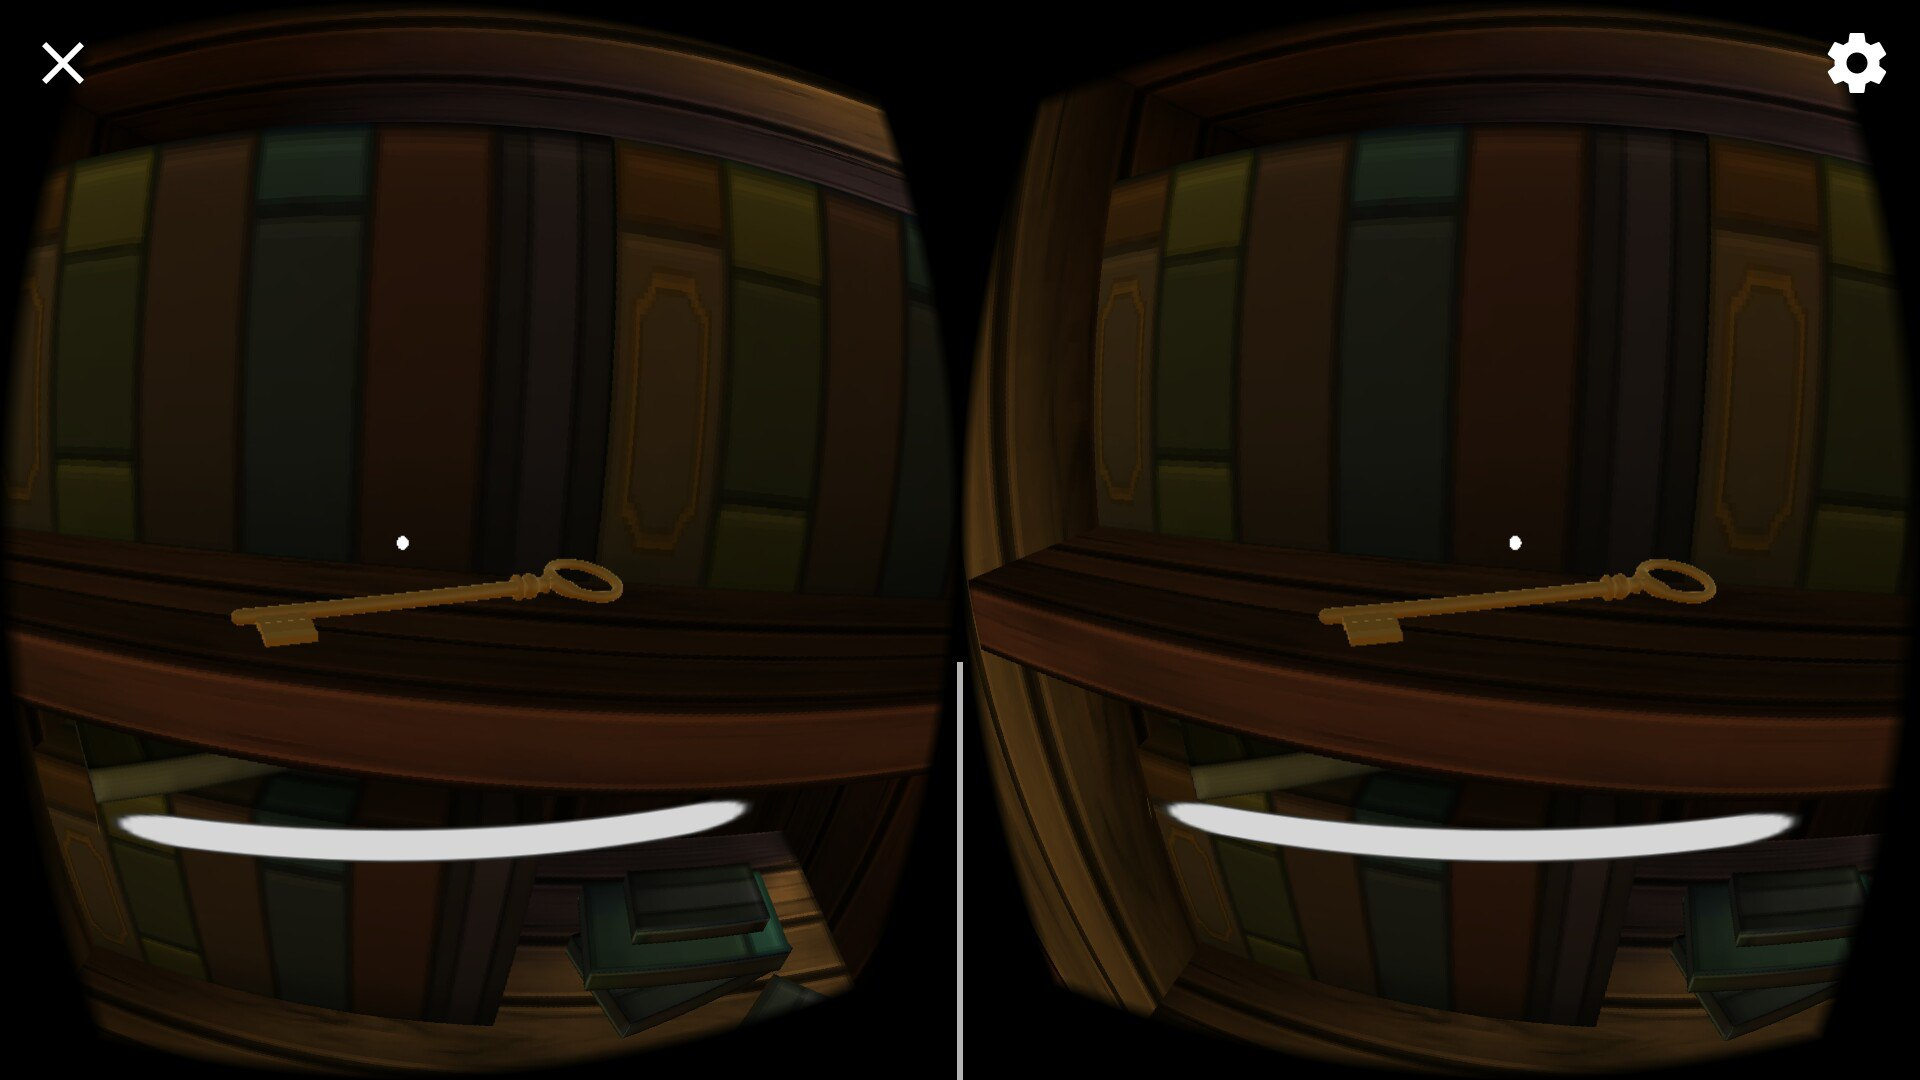
\includegraphics[width=0.8\textwidth]{./screenshots/found_key.jpg}
    \caption{\small{получение ключа.}}
    \label{found_key}
\end{figure} 

\begin{figure}[h!]
    \centering
    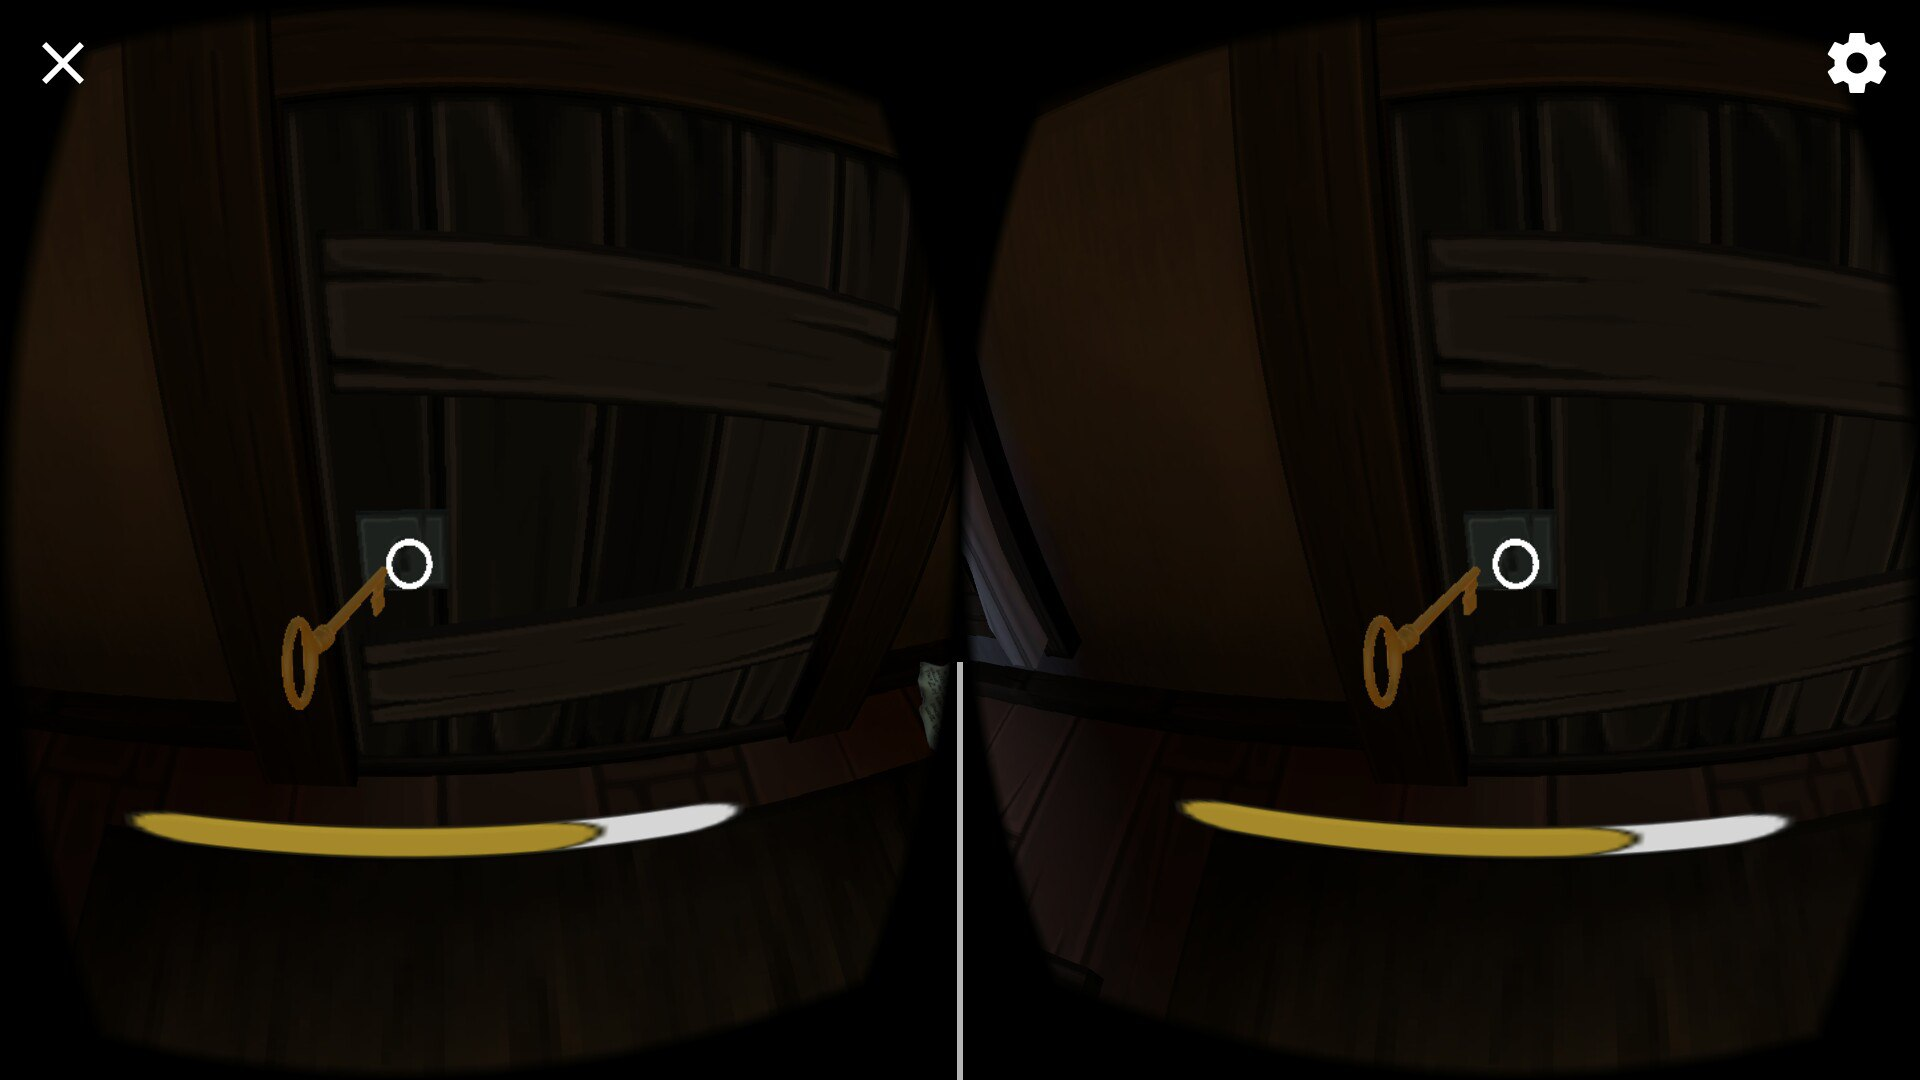
\includegraphics[width=0.8\textwidth]{./screenshots/opening_door.jpg}
    \caption{\small{открытие двери.}}
    \label{opening_door}
\end{figure} 

В скрипте KeyDoorOpener.cs содержится логика открытия двери и загрузки внешнего (снаружи дома) окружения. Изначально оно было отключено из соображений ресурсоэффективности и временных требований к программе. Объекты, которые игрок не наблюдает, не должны прорисовываться. Так же скрипт проигрывает звук отпирания замка, открытия двери.

\begin{small}
    \begin{verbatim}
public GameObject door, final;
private static bool opened = false;
private float timeToOpen = 1F;
public Transform handMountingPosition;

void Start()
{
    opened = false;
    gameObject.GetComponent<BoxCollider>().enabled = false;
}

void Update()
{
    if (handMountingPosition.childCount > 0)
    gameObject.GetComponent<BoxCollider>().enabled = (handMountingPosition.GetChild(0).name.CompareTo("Key") == 0);
}

public void PointerClick()
{
    StartCoroutine(LoadFinalScene());
    StartCoroutine(OpenDoor());
}

private IEnumerator LoadFinalScene()
{
    final.SetActive(true);
    yield return null;
}

private IEnumerator OpenDoor()
{
    if (!opened)
    {
        // play unlock sound
        gameObject.GetComponents<AudioSource>()[0].Play();
        // show input Key and disable current holding Key
        transform.GetChild(0).gameObject.SetActive(true);
        handMountingPosition.GetChild(0).gameObject.SetActive(false);
        yield return new WaitForSeconds(1F);
        transform.GetChild(0).gameObject.SetActive(false);
        transform.GetChild(1).gameObject.SetActive(true);
        gameObject.GetComponents<AudioSource>()[1].Play();
        door.GetComponent<Animation>().Play();
        OpenDoorAndLoadScene.opened = opened = true;
        yield return new WaitForSeconds(timeToOpen);
    }
}

\end{verbatim}
\end{small}

\begin{figure}[h!]
    \centering
    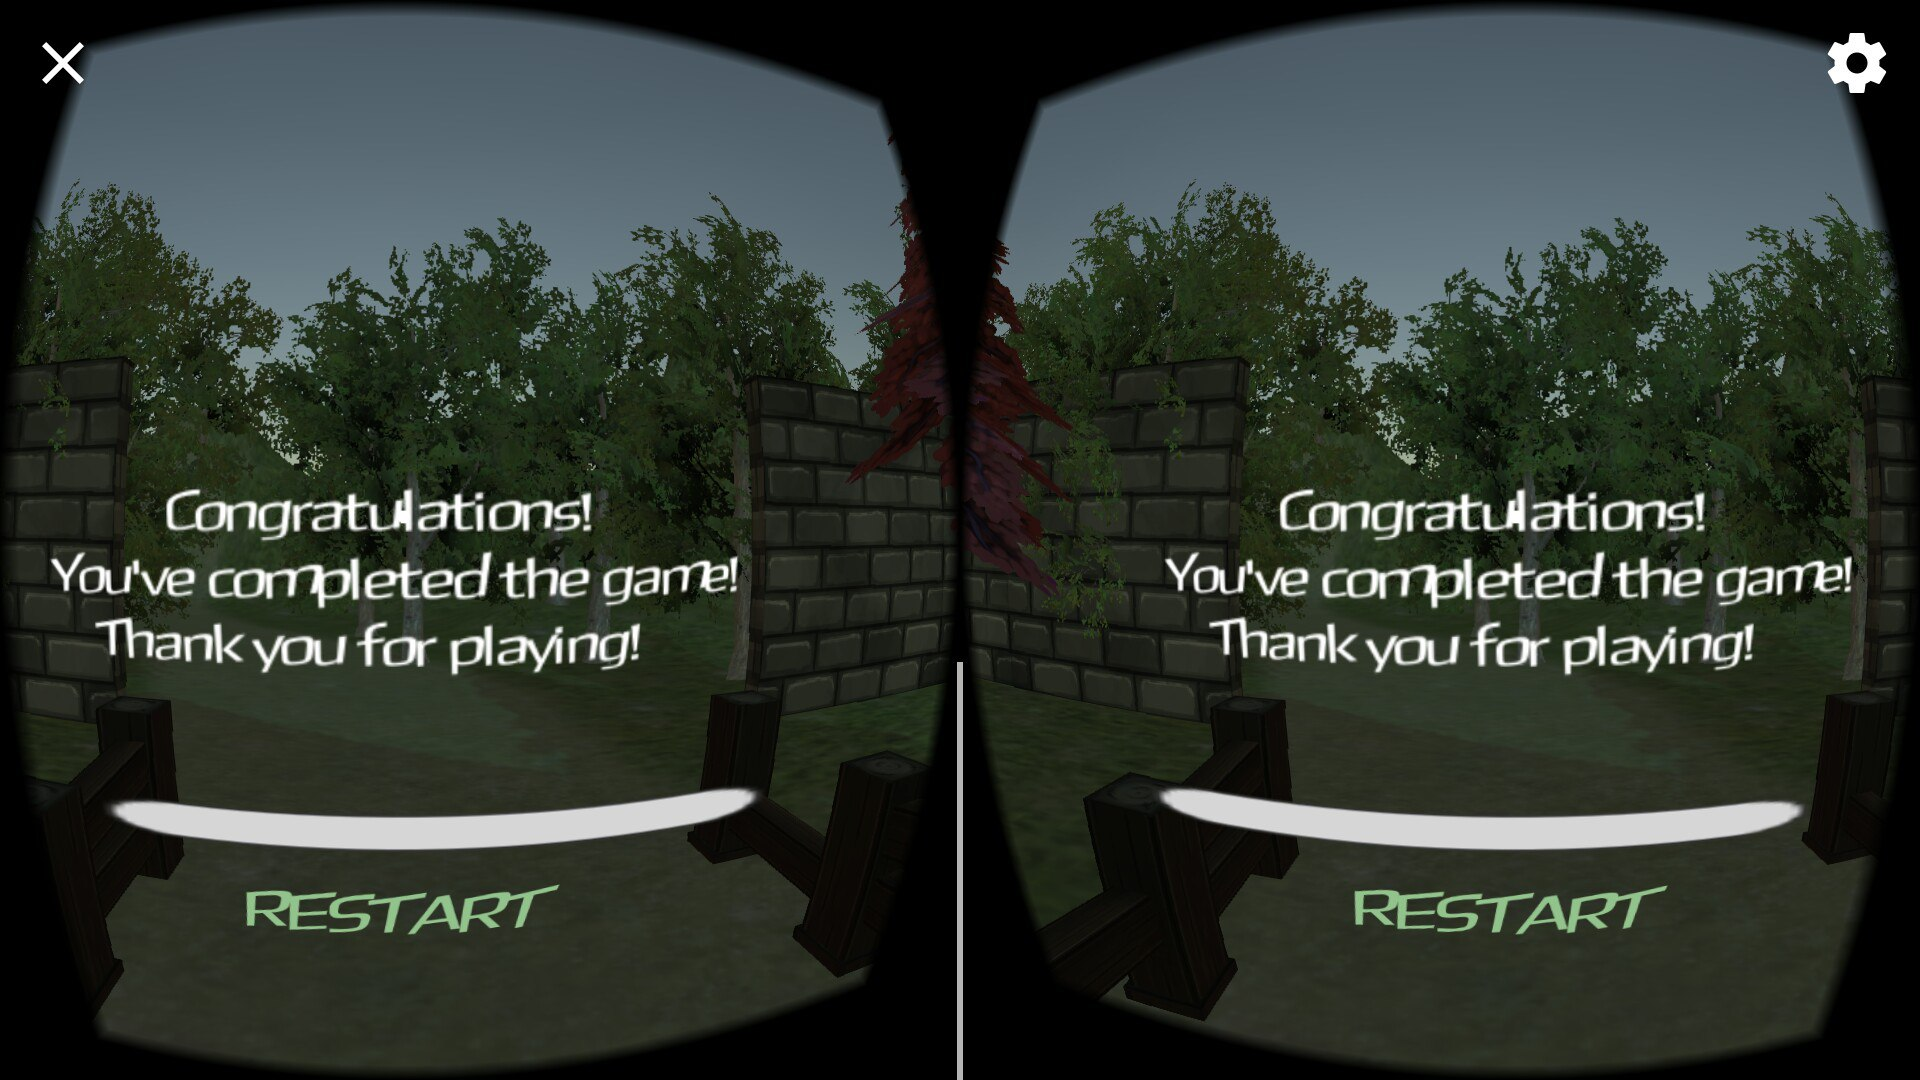
\includegraphics[width=0.8\textwidth]{./screenshots/final.jpg}
    \caption{\small{финал игры.}}
    \label{final}
\end{figure} 

По завершении игры, пользователю будет показано благодарственное сообщение с приглашением пройти игру заново. Происходит этот показ по столкновению персонажа с невидимым объектом, который и вызывает показ.





